\chapter{Mask Training}
\label{chap:chapter2}


\localtableofcontents


\begin{abstract}

  This chapter focuses on the development of lightweight and efficient neural
  networks for image processing tasks, particularly in visual category
  recognition. These lightweight networks are increasingly important for
  intelligent embedded systems with limited computational resources and energy
  availability. Pruning techniques are a popular approach to designing
  lightweight networks, but they require the training of weights. Those weights
  are pruned according to a criterion or associated saliency indicators that are
  trained together with the weights. 
  
  The chapter discusses approaches that seek to extract effective subnetworks by
  pruning large untrained networks, without weight training. A new method, named
  \acf{ASLP}, is proposed to extract effective subnetworks from a large,
  untrained deep neural network using the \acf{STGS} technique. Additionally,
  the \acf{SR} weight rescaling mechanism is introduced. It rescales the weight
  distributions of the selected subnetworks and as a result, improves the
  performance and reduces the number of epochs required for training.
  
  The ASLP method, which integrates the \ac{STGS} sampling technique and the
  \ac{SR} mechanism, is evaluated through a series of experiments on CIFAR-10,
  CIFAR-100, and TinyImageNet datasets. In most cases, ASLP outperforms other
  state-of-the-art methods and consistently surpasses them for various network
  architectures. Further experiments show that the sparsity of the networks
  extracted with \ac{ASLP} can be increased with minimal impact on the
  performance, and also demonstrate the robustness of the method to extreme
  learning rate values and the effectiveness of the \ac{SR} mechanism.\\

  This chapter presents work that has resulted in the publication of the
  following conference article: 
  \bibentry{DBLP:conf/icip/DupontASL22}
  \begin{itemize}
    \item Robin Dupont, Mohammed Amine Alaoui, Hichem Sahbi, and Alice
    Lebois. Extracting effective subnetworks with Gumbel-Softmax. In \textit{2022
    IEEE International Conference on Image Processing, ICIP 2022, Bordeaux,
    France, 16-19 October 2022,} pages 931–935. IEEE, 2022.
  \end{itemize}

\end{abstract}

\section{Introduction and related work}
% region: introduction
Deep neural networks are increasingly utilized for solving various image
processing tasks, especially in the domain of visual category recognition.
While these models have shown significant success, their extensive computational
requirements, memory consumption, and energy consumption are notable
limitations. In light of the emergence of intelligent embedded systems with
restricted computational resources and limited energy availability, there is a
growing need to develop these models with lightweight architectures that
prioritise efficiency while maintaining high accuracy. The aim is to make these
models both lightweight and efficient, which presents a significant challenge for
researchers in the field.\\

Creating small and efficient neural network architectures from scratch is a
viable approach to designing lightweight networks. Despite being smaller than
typical state-of-the-art networks, these networks are still able to achieve good
performance levels. SqueezeNet \cite{DBLP:journals/corr/IandolaMAHDK16} is an
example of such a network, which achieves comparable performance to AlexNet on
ImageNet but with only fifty times fewer parameters. MobileNet
\cite{howard2017mobilenets} and MobileNetV2 \cite{DongMobileNetV2} are also
popular examples of lightweight networks that use depthwise separable
convolution. ShuffleNet \cite{ZhangShuffleNet} and ShuffleNetV2
\cite{MaShuffleNetV2} are other approaches that rely on the grouped convolution
concept and channel shuffling. CondenseNet \cite{huang2018condensenet} leverages
DenseNet-like \cite{huang2017densely} connections together with grouped convolution to pick the most useful features from previous layer maps.\\

Designing efficient lightweight neural networks requires substantial effort from
human experts. These networks are designed from scratch, with a focus on
reducing the number of parameters and computational complexity while maintaining
high accuracy. The design process involves careful consideration of network
architecture, layer types, hyperparameters, and optimization techniques. The
development of such networks, therefore, requires a significant amount of time
and expertise.\\

Another way of obtaining lightweight neural networks is to reduce the size of an
already existing large neural network, through pruning. As discussed in
\cref{chap:chapter1}, pruning methods, either structured or unstructured, are
particularly successful at lightening large neural networks, and seek to remove
connections with the least perceptible impact on classification accuracy.
Structured pruning consists in {\it jointly} removing groups of weights, entire
channels or subnetworks \cite{DBLP:conf/iclr/0022KDSG17,
DBLP:conf/iccv/LiuLSHYZ17}, whereas unstructured pruning aims at removing
weights {\it individually}
\cite{DBLP:conf/nips/HanPTD15,DBLP:journals/corr/HanMD15}.  Unstructured pruning
has witnessed a recent surge in interest in the wake of the \ac{LTH}
\cite{DBLP:conf/iclr/FrankleC19}; an empirical study in
\cite{DBLP:conf/iclr/FrankleC19} demonstrates that large pre-trained networks
encompass lightweight subnetworks, referred to as \textit{\acp{LT}}, which can
achieve comparable performance to the original large network in a similar number
of epochs when trained in isolation with initial weights taken from the large
network. To identify these \acp{LT}, the large network is trained until
convergence, followed by pruning the smallest weights based on their magnitude.
The remaining weights are then rewound to their original value, that is, the
value they had before the training of the large network began. This resulting
subnetwork is known as a \textit{Lottery Ticket}. Another study
\cite{DBLP:conf/iclr/LiuSZHD19} pushes that finding further and concludes that
only the topology of these subnetworks is actually important in order to reach
comparable performances. Authors in \cite{DBLP:conf/iclr/LiuSZHD19} point out
that the weights of the \acp{LT} are not important and can be randomly
initialised, provided that the optimisation procedure is carefully designed.\\

In general, extracting an efficient subnetwork is still an open problem and is
computationally demanding as this amounts to full training of large networks
(until convergence) prior to their pruning. Existing alternatives approach this
problem using early pruning \cite{DBLP:conf/iclr/LeeAT19,
DBLP:conf/iclr/WangZG20,DBLP:conf/nips/TanakaKYG20}, but still require to train
the weights. In contrast to these works, our proposed solution in this chapter
identifies effective subnetworks by training only their topology and without any
weight tuning.\\ 

At first, it seems counterintuitive that there exists a subnetwork in a large
network, and that this subnetwork can achieve compelling performances without
any weight training. This as been first conjectured in
\cite{DBLP:conf/cvpr/RamanujanWKFR20} as the Strong \ac{LTH}. A theoretical
analysis provided evidence that such subnetworks do exist.
\cite{DBLP:conf/icml/MalachYSS20} demonstrate that a neural network of width $d$
and depth $l$ can be approximated by pruning a randomly initialised one that is
a factor $O(d^4l^2)$ wider and twice as deep. The  upper bound on the network
width has latter been improved by \cite{DBLP:conf/nips/OrseauHR20} to
$O(d^2\log(dl))$ under the assumption of a hyperbolic weight distribution. This
upper bound was eventually refined to $O(d\log(dl))$ by
\cite{DBLP:conf/nips/PensiaRNVP20} for a broad class of distributions, including
the uniform distribution which is widely used for weight initialisation \cite{DBLP:conf/iccv/HeZRS15}.\\

Although their existence has been established, no constructive proof has been
provided in order to identify the lightweight and efficient from-scratch
subnetworks. In this context, Zhou et al. \cite{DBLP:conf/nips/ZhouLLY19}
proposed the first attempt to extract efficient subnetworks using stochastic
mask training. A probability of selecting each weight is defined (as the sigmoid
of a mask) and trained using the \ac{STE} \cite{DBLP:journals/corr/BengioLC13}.
During training, weights are frozen and only the masks are allowed to vary.
However, the major drawback of this method resides in the vanishing gradient
issue of the sigmoid which makes mask training numerically challenging.
Ramanujan et al. \cite{DBLP:conf/cvpr/RamanujanWKFR20} proposed another
alternative, based on binarised saliency indicators learned with \ac{STE}, which
selects the most prominent weights in the resulting subnetworks. Nevertheless,
since this method enforces the pruning rate \textit{a priori}, finding the pruning
rate giving the highest performances has to be made through a cumbersome and
time-consuming binary search or grid-search. \\ 

Considering the limitation of the aforementioned related work, we introduce in
this chapter a new stochastic subnetwork selection method based on \ac{GS}.
The latter allows sampling subnetworks whose weights are the most relevant for
classification. The proposed contribution also relies on a new mask
parametrisation, dubbed as \ac{ASLP}, that allows better conditioning of the
gradient and thereby mitigates numerical instability during mask optimisation.
Besides, when combining \ac{ASLP} with a learned weight rescaling mechanism,
training is accelerated and the accuracy of the resulting subnetworks improves
as shown later in experiments.

The rest of this chapter is organized as follows.
% TODO: Completer "chapter organisation"


% endregion: introduction


\section{Extracting Effective Subnetworks with Gumbel-Softmax}
% region: method

Considering the same formalism as in \cref{chap:chapter1}, let $f_\theta$ be a
deep neural network whose weights are defined as $\theta =
\left\{\bm{w}_1,\mathellipsis, \bm{w}_L \right\}$, with $L$ being its depth,
$\bm{w}_\ell \in \mathbb{R}^{d_{\ell} \times d_{\ell-1}}$ its $\ell^\textrm{th}$
layer weights, and $d_\ell$ the dimension of $\ell$. The output of a given layer
$\ell$ is defined as \\

\begin{equation}
  \label{eqn:chap2:layer_eq}
  \mathbf{z}_{\ell} = g_\ell(\bm{w}_\ell \otimes \mathbf{z}_{\ell-1}),
\end{equation}\\

being  $g_\ell$ an activation function and $\otimes$ the usual matrix product.
Without loss of generality, we omit the bias in the definition of
(\ref{eqn:chap2:layer_eq}).

% ------------------------------------------------------------------------------
\subsection{Stochastic Weight Sampling}
\label{sec:chap2:stochastic-sampling}
% region: stochastic-sampling
\indent Given a network $f_\theta$, weight pruning consists in removing
connections in the graph of $f_\theta$. A node in this graph refers to a
neural unit while an edge corresponds to a cross-layer connection. Pruning is
usually obtained by freezing and zeroing out  a subset of weights in $\theta$,
and this is achieved  by multiplying $\bm{w}_\ell$ by a binary mask
$\bm{m}_\ell \in \{ 0,1 \}^{\text{dim}(\bm{w}_\ell)}$. The
binary entries of $\bm{m}_\ell$ are set depending on whether the underlying
layer connections are kept or removed, so \Cref{eqn:chap2:layer_eq} becomes\\

\begin{equation}
  \label{eqn:chap2:pruned_layer_eq}
  \mathbf{z}_{\ell} = g_\ell( (\bm{m}_\ell \odot \bm{w}_\ell ) \otimes \mathbf{z}_{\ell-1} ).
\end{equation}\\

Here $\odot$ stands for the element-wise matrix product. In this definition, the
masks $\{\bm{m}_\ell\}_\ell$ are stochastic and sampled from a Bernoulli
distribution. However, sampling is not a differentiable operation, therefore,
optimising directly $\{{\bm{m}_\ell}\}_\ell$ is not possible. To overcome this
issue, while staying in the \ac{SGD} framework the \acf{STE} technique is
applied together with a reparametrisation of the mask.\\

\noindent\textbf{Straight Through Estimator.} Zhou et
al. \cite{DBLP:conf/nips/ZhouLLY19} consider a Bernoulli parametrisation of
$\{\bm{m}_\ell\}_\ell$ in order to sample masks in
\Cref{eqn:chap2:pruned_layer_eq}. Since sampling is not a differentiable
operation, they rely on the \ac{STE}. It is a technique developed in
\cite{DBLP:journals/corr/BengioLC13} that enables the training of neural
networks with discrete activations, such as binary or quantised activations. The
technique involves using a continuous approximation to the non-differentiable
activation function during forward propagation, and simply passing the gradient
of the loss function through the non-differentiable activation during
backpropagation. This allows for the use of \ac{SGD} to optimise the network,
which was previously not possible with discrete activations. \\

In order to apply \ac{STE} to the problem of Bernoulli stochastic mask
sampling, the definition of $\{\bm{m}_\ell\}_\ell$ is based on another
{\it latent} parametrisation $\{\bm{\hat{m}}_\ell\}_\ell$, detailed
subsequently, and obtained by applying a sigmoid function $\sigma(.)$ to
$\bm{\hat{m}}_\ell$. This allows optimizing $\bm{\hat{m}}_\ell$  using gradient
descent by considering the following surrogate of
\cref{eqn:chap2:pruned_layer_eq} in the backward pass of the backpropagation
algorithm:\\

\begin{equation}
  \label{eqn:chap2:pruned_layer_eq2}
  \mathbf{z}_{\ell} = g_\ell( ( \sigma(\bm{\hat{m}}_\ell) \odot \bm{w}_\ell ) \otimes \mathbf{z}_{\ell-1} ).
\end{equation} \\

\noindent As a result, although masks $\bm{m}_\ell$ are sampled and thus
disconnected from the computation graph (sampling being not differentiable),
their reparametrisation $\bm{\hat{m}}_\ell$ can be updated as if they were used in
the computational graph as in \cref{eqn:chap2:pruned_layer_eq}.\\


\noindent\textbf{Gumbel-Softmax.} In what follows, we consider an alternative to
\ac{STE} based on Gumbel-Softmax \cite{DBLP:conf/iclr/JangGP17} that demonstrate
better performances for differentiable categorical sampling. Gumbel-Softmax is a
technique that can be used to approximate a discrete categorical distribution
with a continuous relaxation. Gumbel-Softmax works by using the Gumbel
distribution to add noise to a categorical distribution and then applying the
Softmax function to obtain a continuous relaxation of the discrete distribution.
The proposed method, dubbed as \ac{STGS}, is based on a variant of \ac{GS}
combined with \ac{STE}. In the forward pass, the softmax of \ac{GS} is replaced
by an argmax operator. Since this operator is not differentiable, the standard
softmax is considered in the backward pass. The argmax operator allows sampling
from a categorical distribution, as the limit of \ac{GS} (\emph{i.e.}, when its
softmax temperature approaches zero). \\

Let $z$ be a categorical random variable, associated with $n$ class probability
distribution $\mathcal{P} = [\pi_1,\dots,\pi_n]$. to sample in a
differentiable manner, the Gumbel-Softmax estimator takes as an input a vector
of log-probabilities \\

\begin{equation}
  \label{eqn:chap2:gumbel-softmax-input}
  \log(\mathcal{P}) =[\log(\pi_1),\dots, \log(\pi_n)] 
\end{equation}\\

then it disrupts the latter with a random additive noise sampled from the Gumbel
distribution, and finally takes the argmax of it, yielding a categorical
variable. More formally, following \cite{DBLP:conf/iclr/JangGP17}, the value $q$
of our categorical variable $z$ is obtained as \\

\begin{equation}
  \label{eqn:chap2:gumbel-softmax-argmax}
  q = \underset{k}{ \text{argmax}} \ [ \log(\pi_k)+g_k ],
\end{equation}\\

with $g_k$ being independent and identically distributed sampled from  the
Gumbel distribution noted $\mathcal{G}(0,1)$.\\

For mask sampling, only two possible outcomes are considered. Either the
corresponding weight is selected and its mask is set to 1, or it is pruned
from the sampled topology and its mask is set to 0. In what follows, and
unless stated otherwise, we omit $\ell$ from $\bm{w}_\ell$ and we write it for
short as $\bm{w}$. Let $\bm{w}_{ij}$ be the weight associated with the i-th and
j-th neurons respectively belonging to layers $\ell-1$ and $\ell$. Since there
are two possible outcomes for the masks define a two-class categorical distribution
$\mathcal{P}_{ij}$ on $\{0,1\}$ as\\

\begin{equation}
    \left\{ \begin{array}{c}
    \mathcal{P}_{ij}(z=1)=\pi_1^{ij} \\ 
    \mathcal{P}_{ij}(z=0)=\pi_2^{ij}
    \end{array} \right.
\end{equation}\\

with $\pi_1^{ij}=p_{ij}$ and $p_{ij}$ being the probability to keep the
underlying connection. Since there are only two mutually exclusive outcomes,
$\pi_2^{ij}=1-p_{ij}$. In other words, keeping the weight $\bm{w}_{ij}$ (or
not) in the sampled topology is a Bernoulli trial with a probability $p_{ij}$.
Considering \Cref{eqn:chap2:gumbel-softmax-argmax}, a binary mask  $\bm{m}_{ij}$
is defined as\\

\begin{equation}
  \label{eqn:chap2:mask_value}
  \bm{m}_{ij} = 1_{\{q_{ij}=1\}}
\end{equation}\\
 
$1_{\{\}}$ being the indicator function and following
\cref{eqn:chap2:gumbel-softmax-argmax}, $q_{ij}$ is\\

\begin{equation}
  \label{eqn:chap2:q_ij_expression}
  q_{ij} = {\text{argmax}_{k \in \{1,2\}}}\big[\log(\pi_k^{ij})+g_k^{ij}\big]
\end{equation}\\

with $\pi^{ij}_1 = p_{ij}$ and $\pi^{ij}_2 = 1-p_{ij}$, the probability for a
weight to be selected or not in the sampled topology, respectively.\\

The proposed \ac{STGS} algorithm enables the learning of probabilities
$p_{ij}$ for each weight $\bm{w}_{ij}$ through \ac{SGD}. However, optimizing
$p_{ij}$ (with \ac{SGD}) raises a major issue. Since the optimisation is not
constrained, $p_{ij}$ can take values larger than 1 or smaller than 0. As a
consequence, it could no longer be interpreted as a probability, moreover,
$\log(p_{ij})$ and $\log(1-p_{ij})$ would also be undefined.\\

On another hand, solving constrained SGD, besides being computationally
expensive and challenging, may result in a worse local minimum. In order to
overcome all these issues, one may consider an alternative reparametrisation
$p_{ij}=\sigma(\bm{\hat{m}}_{ij})$, similar to the reparametrisation in
\cite{DBLP:conf/nips/ZhouLLY19}, with $\bm{\hat{m}}_{ij}$ being a latent mask
variable and $\sigma$ the sigmoid function which bounds $p_{ij}$ in $[0,1]$.
However, this workaround suffers in practice from numerical instability in
gradient estimation and is also computationally demanding. Indeed, the
combination of the log and the sigmoid functions leads to severe numerical
instabilities, that necessitate a cumbersome stabilization by adding
$\varepsilon$ to prevent $p_{ij}$ and $\log(1-p_{ij})$ from being to close to 0.
Furthermore, it is important to note that the above formulation is tremendously
computationally intensive since it necessitates the evaluation of log and
exponential for every mask in the network.\\


\noindent\textbf{Arbitrarily Shifted Log Parametrisation.} In order to solve the
issues related to \ac{STGS} in the context of this chapter, another alternative
is to consider the following expressions for $\log(\mathcal{P}_{ij})$:\\

\begin{equation}
  \label{eqn:chap2:log-probabilities}
  \log(\mathcal{P}_{ij}) =
  \begin{bmatrix}
      \log(p_{ij}) = \bm{\hat{m}}_{ij} \\
      \log(1-p_{ij}) = \log(1-\exp(\bm{\hat{m}}_{ij}))
  \end{bmatrix} 
\end{equation}\\

\noindent and learn the underlying mask $\bm{\hat{m}}_{ij}$. However, this
reparametrisation is also flawed in the same way as the aforementioned sigmoid
reparametrisation, namely: numerically unstable and computationnaly intensive\\

In what follows, we propose an equivalent formulation which turns out to be
highly effective and numerically more stable.  Instead of using the logarithmic
probabilities outlined in \cref{eqn:chap2:gumbel-softmax-input} as the input for
the \ac{STGS} that would eventually lead to the formulation of
\cref{eqn:chap2:log-probabilities}, we adopt the ensuing expression at the
weight level:\\

\begin{equation}
  \label{eqn:chap2:our-input-formulation}
  \begin{bmatrix}
    \bm{\hat{m}}_{ij} \\
    0  \\
  \end{bmatrix}
\end{equation}\\

Here, the second coefficient of the vector, normally representing
$\log(1-p_{ij})$, is set and fixed to 0. It is important to note that this
formulation is not equal to the ones of
\cref{eqn:chap2:gumbel-softmax-input,eqn:chap2:our-input-formulation}. We
interpret this formulation as:

\begin{equation}
  \label{eqn:chap2:our-formulation}
  \begin{bmatrix}
    \bm{\hat{m}}_{ij} \\
    0  \\
  \end{bmatrix}
  = \log\big(\mathcal{P}_{ij}(.)\big) + c =
  \begin{bmatrix}
    \log(p_{ij}) + c \\
    \log(1-p_{ij}) + c\\
  \end{bmatrix},
\end{equation}\\

\noindent In the above expression, instead of using $\log(\mathcal{P}_{ij}(.))$
as an input for \ac{STGS}, we interpret \cref{eqn:chap2:gumbel-softmax-input} as
$\log(\mathcal{P}_{ij}(.)) + c$ , which is the input of the argmax in
\cref{eqn:chap2:gumbel-softmax-argmax}.\\

The constant $c \in \mathds{R}$ does not need to be known.
Adding this constant ensures that even if $\bm{\hat{m}}_{ij} > 0$, we can still interpret $p_{ij}$
as a probability with $\log(p_{ij}) \in ]-\infty,0] \Leftrightarrow p_{ij} \in [0,1]$. This is
enforced by setting the second coefficient of the vector to 0, rather
than computing it explicitly. Although different, the formulation of
\cref{eqn:chap2:our-formulation} is theoretically equivalent to the
aforementioned sigmoid reparametrisation. Indeed, solving the system of
\cref{eqn:chap2:our-formulation} with respect to $\bm{\hat{m}}_{ij}$ yields $p_{ij} =
\sigma(\bm{\hat{m}}_{ij})$ (see \cref{prop:chap2:probability-interpretation}). \\

\begin{proposition}
  [Formulations equivalence]
  \label{prop:chap2:probability-interpretation}
  The formulation in \cref{eqn:chap2:our-formulation} is equivalent to defining
  $p_{ij} = \sigma(\bm{\hat{m}}_{ij})$ with $\sigma$ the sigmoid function,
  provided that $p_{ij}\in ~ ]0,1[$.
\end{proposition}
\vspace*{\baselineskip}

\begin{proof}
  Consider the following system of equations:\\
  $$
  \left\{ 
    \begin{array}{l}
      (1): \bm{\hat{m}}_{ij} = \log(p_{ij})+c\\ 
      (2): 0 = \log(1-p_{ij})+c\\
    \end{array} 
    \right.
  $$\\
  Substracting $(2)$ from $(1)$ yields:\\
  $$ (1) - (2) \Leftrightarrow \bm{\hat{m}}_{ij} = \displaystyle\log\left( \frac{p_{ij}}{1 - p_{ij}} \right)$$\\
  $$ \Leftrightarrow \log\left(\frac{1-p_{ij}}{p_{ij}} \right) = -
  \bm{\hat{m}}_{ij}$$\\
  $$ \Leftrightarrow \frac{1}{p_{ij}} - 1 = \exp(-\bm{\hat{m}}_{ij})$$\\
  $$ \Leftrightarrow \frac{1}{p_{ij}} = \exp(-\bm{\hat{m}}_{ij}) + 1$$\\
  $$ \Leftrightarrow p_{ij} = \frac{1}{\exp(-\bm{\hat{m}}_{ij}) + 1}$$\\
  $$ \Leftrightarrow p_{ij} = \sigma(\bm{\hat{m}}_{ij})$$\\

\end{proof}


Differently put, the formulation in \cref{eqn:chap2:our-formulation} considers a
reparametrisation $\bm{\hat{m}}_{ij} = \log(p_{ij})+c$ and $\log(1-p_{ij})+ c =0$ which is strictly
equivalent to the sigmoid one while being computationally more efficient and
also numerically stable.\\

\Cref{prop:chap2:probability-interpretation} assumes that $p_{ij}\in ~ ]0,1[$.
In practice, this is never a problem as $\bm{\hat{m}}_{ij}$ are initialised to 0
(see \cref{sec:chap2:experiments}) and because of the sigmoid function, the
gradients become vanishingly small when $\bm{\hat{m}}_{ij}$ deviates from 0,
which practically prevents reaching $\pm\infty$ and thus 0 or 1 for $p_{ij}$.\\

A crucial point to consider is that adding any arbitrary constant $c$ to each
coefficient of the log-probability vector does not change the outcome of
Gumbel-Softmax sampling. This is because it does not alter the outcome of the
argmax function, which remains unchanged regardless of the value of $c$,
provided that the same value $c$ is added to both coefficients, which is the case
in our formulation (\emph{c.f.} \cref{eqn:chap2:our-formulation}). The
presence of this constant $c$, whose value is arbitrary, that shifts the
log-probabilities of our probability parametrisation gives the name of the
method: \acl{ASLP}.\\ 

% endregion: stochastic-sampling


\subsection{Smart Weight rescaling}
\label{sec:smart-rescale}
% region: smart rescaling
Subnetwork selection may disrupt the dynamic of the forward pass
\cite{DBLP:conf/iccv/HeZRS15,DBLP:conf/cvpr/RamanujanWKFR20}, and thereby
requires adapting weights accordingly. \cite{DBLP:conf/iccv/HeZRS15} establish
that the variance of the initial weight distribution has a critical impact on
the network performances. Since in the context of this chapter, the weights are
not trained, it is all the more important to address this issue. The pruning of
the weights changes the apparent weight distribution and therefore its
statistics.\\

\ac{DWR} \cite{DBLP:conf/nips/ZhouLLY19}, and scaled Kaiming distribution
\cite{DBLP:conf/cvpr/RamanujanWKFR20} are two known mechanisms that adapt the
weights of the selected subnetworks to circumvent the issue mentioned above.
However, some of these heuristics, besides being handcrafted, rely on the
strong assumption that rescaling should be proportional to the pruning rate.\\

In what follows, we consider a new weight adaptation mechanism, referred to as
\ac{SR}. Instead of handcrafting this rescaling factor proportionally
to the pruning rate (as achieved for instance in
\cite{DBLP:conf/nips/ZhouLLY19}), \ac{SR} is learned layerwise and provides an
effective (and also efficient) way to adapt the dynamic of the forward pass
without retraining the entire weights of the selected subnetwork. This
rescaling ends up reducing the number of epochs needed to reach convergence and
also improving accuracy (to some extent) as shown later in \cref{sec:chap2:experiments}. \\

With SR, the $\ell$-th layer network output becomes \\

  \begin{equation}
   \mathbf{z}_{\ell} = g_\ell(s_\ell \times (\bm{m}_\ell \odot \bm{w}_\ell) \otimes \mathbf{z}_{\ell-1}),
  \end{equation}\\

\noindent where $s_\ell$ refers to the rescaling factor  of the $\ell$-th
layer (see also algorithm~\ref{alg:chap2:ASLP}). Smart Rescale increases
the flexibility of subnetwork selection and adaptation compared to DWR (which
is bound to the pruning rate). Moreover, scaling factors obtained with SR
vary smoothly --- and this makes training more stable with stochastic
gradient descent (SGD) --- compared to the ones obtained with DWR which are
again set to the observed {\it pruning rates}, and changes of the latter are
more abrupt due to stochastic mask sampling. \\

% endregion: smart rescaling


\subsection{Overview}
% region: overview
Our approach integrates the \acl{STGS} sampling technique and the \acl{SR}
mechanism, resulting in a comprehensive method termed \acf{ASLP}. This strategy
constructs lightweight neural networks by sampling topologies from a large,
untrained network and learns the probability of selecting each weight.
Probabilities are determined using \acl{SGD} in conjunction with a standard loss
function, specifically cross-entropy loss for image classification tasks. The
training procedure for our method is detailed in \Cref{alg:chap2:ASLP}. Unless
otherwise noted, this procedure is implemented in
\cref{sec:chap2:experiments}.\\

The core differences between our approach and standard pruning pipelines are
illustrated in \Cref{fig:chap2:our-pipeline,fig:chap2:standard-pipeline}. As
highlighted in \Cref{fig:chap2:our-pipeline}, our method focuses exclusively on
topology selection without weight training, whereas conventional pruning
pipelines rely on weight training and subsequent fine-tuning.\\


\begin{figure}
\centering
\subfloat[Our pruning pipeline\label{fig:chap2:our-pipeline}]{
  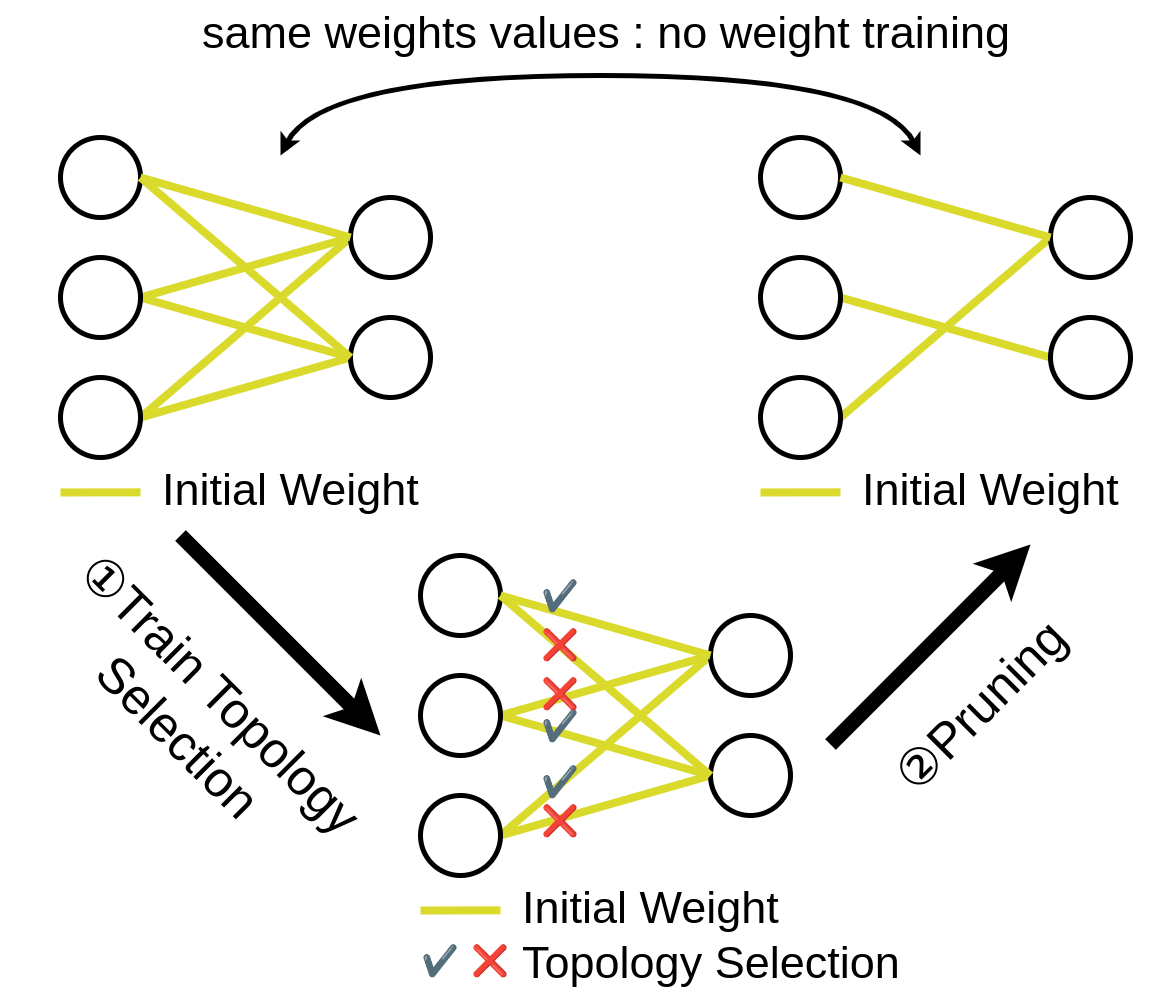
\includegraphics[width=0.4\textwidth]{chapter_2/assets/our_pruning_pipeline.png}}
  \vspace{0.10\textwidth}
  \subfloat[Standard pruning pipelines \label{fig:chap2:standard-pipeline}]{
    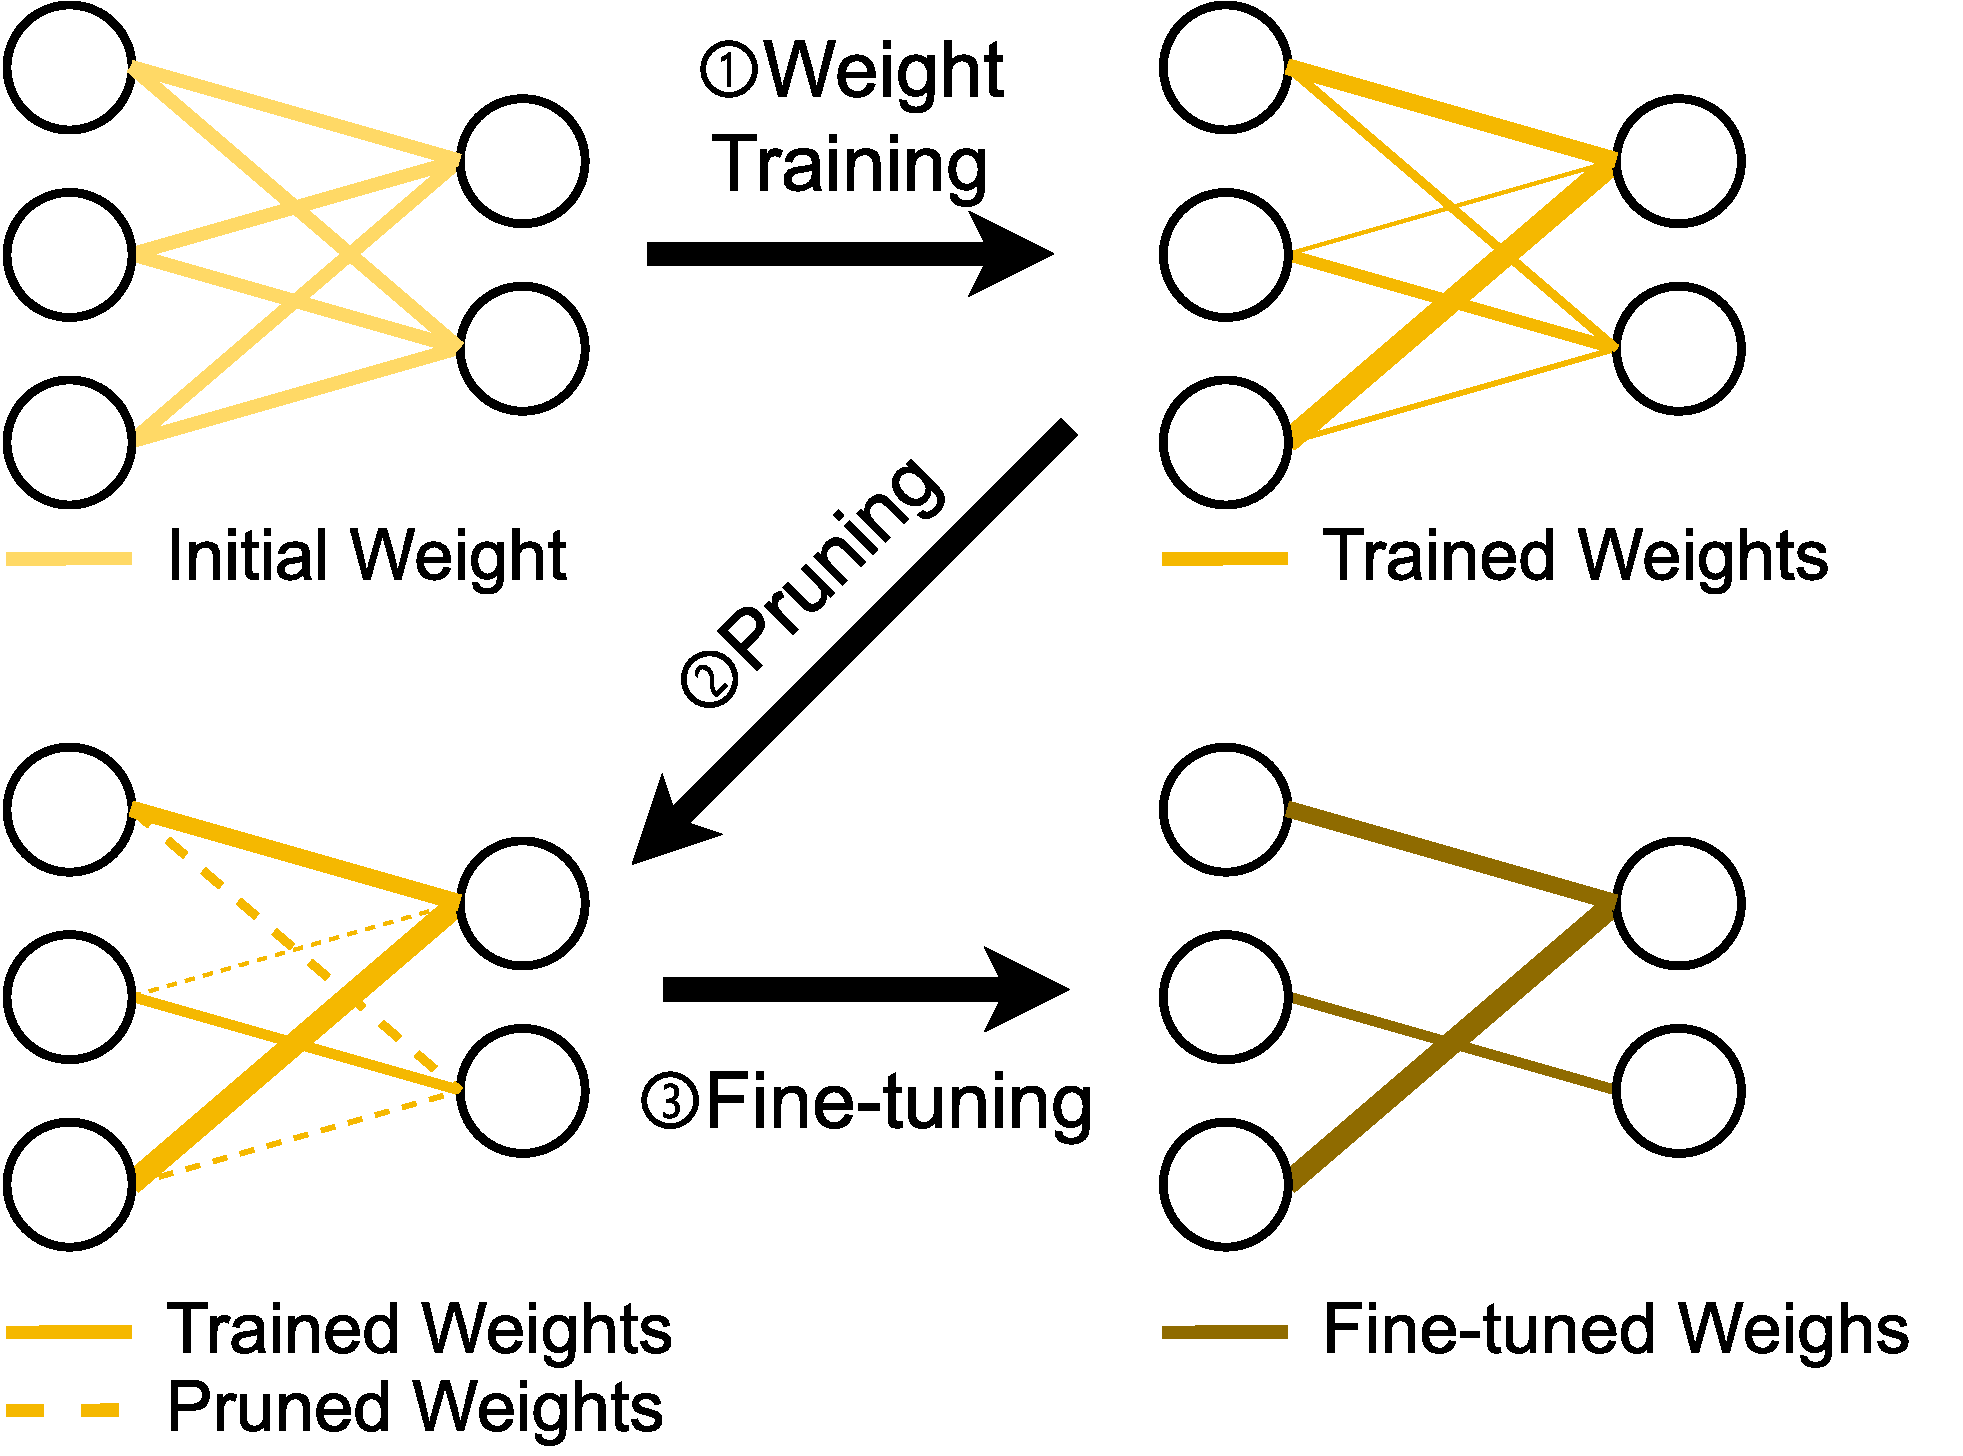
\includegraphics[width=0.4\textwidth]{chapter_2/assets/standard_pruning_pipeline.pdf}}
    \caption{Overview of our pruning pipeline and standard pruning pipelines.
    Our pipeline perfoms topology selection only: weights are not trained. 
    On the contrary, standard pruning pipelines rely on weight training and fine-tuning.}
\end{figure}


\begin{algorithm}
  \caption{Our training procedure}
  \label{alg:chap2:ASLP}
  \begin{algorithmic}
  \REQUIRE Dataset $\mathcal{D} = \{\mathcal{X}, \mathcal{Y}\}$, network $f$,
  weights $\theta$, masks $\bm{\hat{m}}$, number of epochs $n$, learning rate $\eta$
  \FOR{$t = 1$ to $n$}
      \FOR{each $(x,y) \in \mathcal{D}$}
        \STATE
        $q_{i,j} \gets \text{argmax} 
        \begin{bmatrix}
          \bm{\hat{m}}_{i,j} + g_{i,j} \\
          0 + g'_{i,j}\\
        \end{bmatrix}$ \COMMENT{Sampling of a topology}    
        \STATE $m_{ij} \gets 1_{\{q_{ij}=1\}}$
      \COMMENT{Giving the masks $\bm{m}_{i,j}$ their values} 
          
      \STATE $\hat{y} = f(x; \theta_t)$ \COMMENT{Computing the output of the network}
          \STATE ${\cal L}\big(f_\theta(\{{\bf x}_k\}_k;
          \{s_\ell (\bm{m}_\ell \odot \bm{w}_\ell)\}_\ell),\{{\bf y}_k\}_k\big)$ 
          \COMMENT{Computing the loss with masked weights and SR}
          \STATE $\bm{\hat{m}}_{t+1} = \bm{\hat{m}}_t - \eta \nabla_{\bm{\hat{m}}} \mathcal{L}$ \COMMENT{Backpropagate the loss and update the masks}
      \ENDFOR
  \ENDFOR
  \RETURN Network $f$ with unchanged weights $\theta$ and trained masks $\bm{\hat{m}}$.
  \end{algorithmic}
  \end{algorithm}

% endregion: overview

% endregion: method

\section{Experiments and results}
\label{sec:chap2:experiments}
% region: experiments


In this section, we present a series of experiments designed to evaluate the
efficacy of our proposed method, as well as to investigate the influence of
various parameters and configurations. To accomplish this, we employ the same
networks and datasets previously introduced in \cref{chap:chapter1}. The
datasets utilised include CIFAR-10, CIFAR-100, and TinyImageNet. They are
described in \cref{sec:chap1:experiments}. Unless stated otherwise, on each
table we report the test accuracy, given in percentages (plus or minus the
standard deviation), evaluated on the test set of the said datasets. Values are
obtained by averaging 5 independent runs. The architectures considered are
Conv2, Conv4, Conv6, VGG16, ResNet-20, and ResNet-18. Excluding Conv2 and Conv6,
these networks are described in \cref{sec:chap1:experiments}. Conv2 and Conv6
are modified versions of the Conv4 architecture, featuring 2 and 6 convolutional
layers, respectively, instead of the original 4 layers. The number of parameters
for these architectures is provided in \cref{tab:chap2:conv_num_params}.
Although these networks, introduced by \citeauthor{DBLP:conf/iclr/FrankleC19},
are less common in the literature, we use them since they are also used by the
methods we compare ours to.\\

\begin{table}[htbp]
  \centering\begin{tabular}{lccc}
    \cmidrule[\heavyrulewidth]{2-4}
                         & \textbf{Conv2}     & \textbf{Conv4}     & \textbf{Conv6}     \\ \toprule
    Number of Parameters & 4,301,642 & 2,425,930 & 2,262,602 \\ \bottomrule
    \end{tabular}
  \caption{Number of parameters for the Conv2, Conv4 and Conv6 architectures, when used with the CIFAR-10 dataset}
  \label{tab:chap2:conv_num_params}
\end{table}




\subsection{Performances}
\label{sec:chap2:performances}

To demonstrate the efficacy of our method in a standard image classification
scenario, we compare our approach with state-of-the-art methods, specifically
Edge-popup \cite{DBLP:conf/cvpr/RamanujanWKFR20} and Supermask
\cite{DBLP:conf/nips/ZhouLLY19}. We re-implemented both methods in PyTorch
\cite{DBLP:conf/nips/PaszkeGMLBCKLGA19} and employed a uniform training
procedure for all methods: networks are trained for 1000 epochs with a fixed
learning rate of 50 (except for Edge-popup, which utilises a learning rate of
0.1). The learning rate of \ac{SR} is set to $1\times10^{-3}$, and  neither
weight decay nor $\ell_2$ regularisation is applied. This section examines
several configurations initially presented in \cite{DBLP:conf/nips/ZhouLLY19},
which encompass combinations of techniques or enhancements employed for method
evaluation. The various techniques include data augmentation, the application of
\ac{WR}, and the use of \ac{SC} weight distribution.\\

\noindent\textbf{Data augmentation.} Although \cite{DBLP:conf/nips/ZhouLLY19}
did not introduce data augmentation, it is a widely accepted practice in image
classification and is generally applied even if not explicitly mentioned in the
article. Consequently, we consider two configurations: with (w/) and without
(w/o) data augmentation. The data augmentation we apply has been observed in
various state-of-the-art implementations and is the following: first, images
are padded with zeroes, expanding them to one-eighth of their initial size.
Next, a random crop of the original size is extracted from the enlarged image.
Lastly, a random horizontal flip is performed.\\

\noindent\textbf{Weight Rescaling (WR).} Each method discussed in this section
incorporates its own weight rescaling technique: \ac{DWR} for
\cite{DBLP:conf/nips/ZhouLLY19}, \ac{FS} for
\cite{DBLP:conf/cvpr/RamanujanWKFR20}, and \ac{SR} for \ac{ASLP}. All of these
techniques are denoted as \ac{WR} in this section.\\ 

\noindent\textbf{Signed Constant Distribution (SC).} The signed constant distribution
was introduced by \cite{DBLP:conf/nips/ZhouLLY19}. Weights sampled from this
distribution can take only two values: $-\sigma$ and $\sigma$, where $\sigma$
represents the standard deviation of the weight tensor upon initialization using
the widely adopted Kaiming initialization \cite{DBLP:conf/iccv/HeZRS15}.
\citeauthor{DBLP:conf/nips/ZhouLLY19} report that it improves performances over
the standard weight initialisation scheme. \\


After training the selection probabilities of the neural network's weights, a
pruning step is applied to extract a subnetwork for the large initial network.
Our pruning strategy is based on thresholding the weight probability selection:
a weight is selected if its probability of selection is above 0.5, otherwise, it
is pruned. In other words, the weight is kept if the binary event of keeping a
connection is more likely than its removal. This means retaining the weight
$\bm{w}_{i,j}$ if $\bm{\hat{m}}_{i,j} > 0$ and setting it to zero otherwise. We
refer to this pruning method as \textit{thresholding}. As a matter of comparison,
we also consider the setting in \citeauthor{DBLP:conf/nips/ZhouLLY19} which is
an averaging strategy to evaluate Supermask performance. It consists in sampling
ten different topologies and averaging their test accuracies. We refer to this
pruning strategy as \textit{averaging}. Edge-popup does not require pruning as it
is integrated into the forward pass. \\

Overall, the analysis of our ASLP method's results shows that ASLP outperforms
both Edge Popup and Supermask methods on CIFAR-10 and CIFAR-100 datasets, a
trend consistent across all tested networks, including Conv2, Conv4, Conv6,
VGG16, and ResNet20. Notably, our \textit{thresholding} pruning strategy
demonstrated superior performance compared to Supermask's \textit{averaging}
approach. However, it should be noted that on the CIFAR-100 dataset, our method
slightly underperforms compared to Edge Popup for the Conv6 network.\\

Remarkably, for larger networks such as VGG16 and ResNet-20, our ASLP method
employing the \textit{thresholding} strategy also consistently surpasses all
other methods. Although, when evaluating the ResNet-18 network with the
TinyImageNet dataset, our method appears to be less optimal than others. \\

% =========================================================

We put forth several hypotheses to account for the reduced performance. First,
the ResNet-18 architecture employed is the standard PyTorch implementation
\cite{pytorch_resnet18}, designed for the ImageNet dataset
\cite{deng2009imagenet}. As a result, it is tailored for $224 \times 224$ pixel
images, while TinyImageNet images are only $64 \times 64$ pixels. With a
smaller input image size, each pixel encompasses a larger area of the input
space, and an overly large receptive field for a smaller image like TinyImageNet
may lead to the loss of crucial spatial information. We opted against upscaling
TinyImageNet images to $224 \times 224$ as a preprocessing step in order to
prevent an exponential increase in computational cost.\\

Secondly, the ResNet-18 network is among the largest networks we examined (refer
to \cref{tab:chap1:networks_size}). As a result, there are numerous possible
weight combinations and subnetworks. Viewing \ac{ASLP} as a Neural Architecture
Search method, the search space for ResNet-18 is considerably larger than for
the Conv\{2,4,6\} networks. Nevertheless, the number of sampled topologies is only
equal to the product of the number of batches and the number of epochs during
which the network is trained. Since the number of images in the CIFAR and
TinyImageNet datasets are of the same order of magnitude (see
\cref{tab:chap1:datasets}), and the number of evaluated topologies is roughly the
same. This may be sufficient to explore the search space for Conv\{2,4,6\}
networks but it might not be enough for a ResNet-18 network.\\

However, this hypothesis warrants further clarification. Indeed, the VGG16
network has more parameters than the ResNet-18, but \ac{ASLP} achieves superior
results compared to other methods on this architecture. We suggest the following
explanation: Although the VGG16 has more parameters, it has fewer weights in its
fully connected layers since the dataset it is evaluated on has fewer classes.
Thus, the search space for the fully connected part of the VGG network is much
smaller than on the ResNet-18 network. The final fully connected layers of a
neural network play a crucial role in determining its overall performance and
accuracy in predicting outcomes.\\

%=============================================




% region: perf-tables
\begin{table}[htbp]
  \centering
  \resizebox{16.5cm}{!} {
    \begin{tabular}{llcccccccc}
      \cmidrule[\heavyrulewidth]{3-10}
        &  & \multicolumn{4}{c}{\textbf{w/ data augmentation}} & \multicolumn{4}{c}{\textbf{w/o augmentation}} \\
       &  &  $\varnothing$ & \textbf{SC} & \textbf{WR} & \textbf{WR+SC} & $\varnothing$ & \textbf{SC} & \textbf{WR} & \textbf{WR+SC} \\
      \toprule

      % Conv 2 results
      \multirow{12}{*}{} \multirow{4}{*}{\textbf{Conv2}} & ASLP (thresholding) & \textbf{75.70 $\pm$ 0.30} & \textbf{75.81 $\pm$ 0.69} & \textbf{76.48 $\pm$ 0.68} & \textbf{76.92 $\pm$ 0.24} & \textbf{68.24 $\pm$ 0.14} &\textbf{ 68.11 $\pm$ 0.64} & \textbf{66.84 $\pm$ 0.46} & \textbf{66.05 $\pm$ 0.93} \\
        & ASLP (averaging)& 75.42 $\pm$ 0.25 & 75.50 $\pm$ 0.56 & 76.05 $\pm$ 0.44 & 76.44 $\pm$ 0.19 & 68.09 $\pm$ 0.35 & 67.69 $\pm$ 0.52 & 65.79 $\pm$ 0.65 & 65.35 $\pm$ 0.83 \\
        & \cite{DBLP:conf/nips/ZhouLLY19} (averaging)& - & - & - & - & 67.12 $\pm$ 0.25 & 66.34 $\pm$ 0.41 & 56.71 $\pm$ 2.99 & 56.26 $\pm$ 1.64 \\
        & \cite{DBLP:conf/cvpr/RamanujanWKFR20} ($k=50\%$) & 74.18 $\pm$ 0.76 & 75.19 $\pm$ 0.56 & 74.51 $\pm$ 0.31 & 75.45 $\pm$ 0.44 & - & - & - & - \\
      \midrule

      % Conv 4 results
       \multirow{4}{*}{\textbf{Conv4}} & ASLP (thresholding) & \textbf{83.03 $\pm$ 0.31} & \textbf{83.73 $\pm$ 0.46} & \textbf{83.59 $\pm$ 0.29} & \textbf{84.06 $\pm$ 0.31} & \textbf{71.64 $\pm$ 0.36} & \textbf{69.74 $\pm$ 1.37} & \textbf{72.85 $\pm$ 0.48} & \textbf{72.08 $\pm$ 0.62} \\
        & ASLP (averaging)& 82.29 $\pm$ 0.25 & 83.22 $\pm$ 0.56 & 82.79 $\pm$ 0.30 & 83.46 $\pm$ 0.49 & 70.88 $\pm$ 0.47 & 68.77 $\pm$ 1.42 & 71.82 $\pm$ 0.53 & 71.09 $\pm$ 0.69 \\
        & \cite{DBLP:conf/nips/ZhouLLY19} (averaging)& - & - & - & - & 68.09 $\pm$ 0.84 & 67.48 $\pm$ 0.52 & 58.13 $\pm$ 2.39 & 53.84 $\pm$ 5.00 \\
        & \cite{DBLP:conf/cvpr/RamanujanWKFR20} ($k=50\%$) & 82.38 $\pm$ 0.29 & 83.61 $\pm$ 0.38 & 81.71 $\pm$ 0.59 & 83.55 $\pm$ 0.32 & - & - & - & - \\
      \midrule

      % Conv 6 results
       \multirow{4}{*}{\textbf{Conv6}} & ASLP (thresholding) & \textbf{84.98 $\pm$ 0.33} & \textbf{86.49 $\pm$ 0.36} & \textbf{85.32 $\pm$ 0.27} & \textbf{86.21 $\pm$ 0.34} & \textbf{73.32 $\pm$ 0.42} & \textbf{69.83 $\pm$ 1.46} & \textbf{76.20 $\pm$ 0.91} & \textbf{75.30 $\pm$ 0.89} \\
        & ASLP (averaging)& 84.24 $\pm$ 0.28 & 85.67 $\pm$ 0.34 & 84.51 $\pm$ 0.35 & 85.49 $\pm$ 0.38 & 72.62 $\pm$ 0.57 & 69.53 $\pm$ 1.68 & 75.24 $\pm$ 0.69 & 74.50 $\pm$ 0.96 \\
        & \cite{DBLP:conf/nips/ZhouLLY19} (averaging) & - & - & - & - & 70.71 $\pm$ 0.98 & 69.16 $\pm$ 1.92 & 44.77 $\pm$ 17.02 & 36.59 $\pm$ 15.32 \\
        & \cite{DBLP:conf/cvpr/RamanujanWKFR20} ($k=50\%$) & 84.67 $\pm$ 0.35 & 85.87 $\pm$ 0.13 & 84.37 $\pm$ 0.58 & 85.84 $\pm$ 0.51 & - & - & - & - \\
      \bottomrule
    \end{tabular}
  }
  \caption{Comparison of ASLP's performance with Edge-Popup and Supermask
  \cite{DBLP:conf/cvpr/RamanujanWKFR20,DBLP:conf/nips/ZhouLLY19} on CIFAR10
  using various configurations. We use the configurations tested by the author
  of the aforementioned articles. Performance measures reported are accuracy and
  are presented with and without data augmentation, weight rescaling (WR), and
  the signed constant weight distribution (SC). We report performances for both
  \textit{thresholding} and \textit{averaging} setups for our method. For edge-popup, we use
  the best $k$ value for Conv\{2,4,6\} reported in
  \cite{DBLP:conf/cvpr/RamanujanWKFR20}.  Across all setups, our method ASLP
  outperforms Edge-Popup and Supermask}
  \label{tab:chap2:con_performances_comparison_cifar10}
  
\end{table}



\begin{table}[htbp]
  \centering
  \resizebox{16.5cm}{!}{
    \begin{tabular}{lllllllllll}
      \cmidrule[\heavyrulewidth]{3-10}
      &  & \multicolumn{4}{c}{\textbf{w/ data augmentation}} & \multicolumn{4}{c}{\textbf{w/o augmentation}} \\
      &  &  $\varnothing$ & \textbf{SC} & \textbf{WR} & \textbf{WR+SC} & $\varnothing$ & \textbf{SC} & \textbf{WR} & \textbf{WR+SC} \\
      \toprule
      \multirow{12}{*}{}
      \multirow{4}{*}{\textbf{Conv2}} & ASLP (thresholding) & \textbf{38.64 $\pm$ 0.92} & 38.31 $\pm$ 0.75 & \textbf{41.81 $\pm$ 0.84} & \textbf{42.06 $\pm$ 0.76} & \textbf{38.72 $\pm$ 0.59} & 38.64 $\pm$ 1.23 & \textbf{42.42 $\pm$ 0.30} & \textbf{41.95 $\pm$ 0.68} \\
      & ASLP (averaging) & 38.49 $\pm$ 0.61 & 38.18 $\pm$ 0.81 & 41.12 $\pm$ 0.66 & 41.17 $\pm$ 0.54 & 38.40 $\pm$ 0.81 & \textbf{38.71 $\pm$ 1.05} & 41.66 $\pm$ 0.39 & 41.42 $\pm$ 0.55 \\
      & \cite{DBLP:conf/nips/ZhouLLY19} (averaging) & - & - & - & - & 38.09 $\pm$ 1.03 & 37.28 $\pm$ 0.47 & 26.03 $\pm$ 2.23 & 23.49 $\pm$ 1.36 \\
      & \cite{DBLP:conf/cvpr/RamanujanWKFR20} ($k=50\%$) & 38.47 $\pm$ 0.46 & \textbf{39.83 $\pm$ 0.46} & 38.57 $\pm$ 0.59 & 39.87 $\pm$ 0.78 & - & - & - & - \\
      \midrule

      \multirow{4}{*}{\textbf{Conv4}} & ASLP (thresholding) & \textbf{47.78 $\pm$ 1.18} & 49.33 $\pm$ 0.77 & \textbf{50.33 $\pm$ 0.39} & \textbf{51.49 $\pm$ 0.43} & \textbf{47.56 $\pm$ 0.36} & \textbf{49.30 $\pm$ 0.54} & \textbf{50.39 $\pm$ 0.58} & \textbf{51.16 $\pm$ 0.94} \\
      & ASLP (averaging) & 47.18 $\pm$ 1.17 & 48.78 $\pm$ 0.79 & 49.39 $\pm$ 0.30 & 50.17 $\pm$ 0.50 & 46.89 $\pm$ 0.52 & 48.74 $\pm$ 0.47 & 49.55 $\pm$ 0.57 & 50.23 $\pm$ 0.87 \\
      & \cite{DBLP:conf/nips/ZhouLLY19} (averaging) & - & - & - & - & 45.84 $\pm$ 1.01 & 47.72 $\pm$ 0.75 & 27.70 $\pm$ 2.41 & 27.53 $\pm$ 5.20 \\
      & \cite{DBLP:conf/cvpr/RamanujanWKFR20} ($k=50\%$) & 47.75 $\pm$ 0.63 & \textbf{50.16 $\pm$ 0.47} & 48.20 $\pm$ 0.72 & 50.02 $\pm$ 0.65 & - & - & - & - \\
      \midrule

      \multirow{4}{*}{\textbf{Conv6}} & ASLP (thresholding) & 51.09 $\pm$ 0.92 & 53.00 $\pm$ 0.52 & \textbf{51.70 $\pm$ 0.48} & 52.85 $\pm$ 0.50 & \textbf{51.43 $\pm$ 0.41} & \textbf{53.10 $\pm$ 0.27} & \textbf{51.52 $\pm$ 0.35} & \textbf{53.22 $\pm$ 0.54} \\
      & ASLP (averaging) & 50.22 $\pm$ 1.09 & 51.72 $\pm$ 0.73 & 50.56 $\pm$ 0.33 & 51.59 $\pm$ 0.24 & 50.47 $\pm$ 0.42 & 52.00 $\pm$ 0.27 & 50.38 $\pm$ 0.33 & 51.82 $\pm$ 0.34 \\
      & \cite{DBLP:conf/nips/ZhouLLY19} (averaging) & - & - & - & - & 49.19 $\pm$ 0.75 & 50.66 $\pm$ 0.47 & 2.54 $\pm$ 1.63 & 9.21 $\pm$ 5.50 \\
      & \cite{DBLP:conf/cvpr/RamanujanWKFR20} ($k=50\%$) & \textbf{51.13 $\pm$ 0.39} & \textbf{53.48 $\pm$ 0.51} & 51.06 $\pm$ 1.11 & \textbf{54.01 $\pm$ 0.35} & - & - & - & - \\
      \bottomrule
    \end{tabular}
  } \caption{Comparison of ASLP's performance with Edge-Popup and Supermask
  \cite{DBLP:conf/cvpr/RamanujanWKFR20,DBLP:conf/nips/ZhouLLY19} on CIFAR100
  using various configurations. We use the configurations tested by the author
  of the aforementioned articles. Performance measures reported are accuracy and
  are presented with and without data augmentation, weight rescaling (WR), and
  the signed constant weight distribution (SC). We report performances for both
  \textit{thresholding} and \textit{averaging} setups for our method. For edge-popup, we use
  the best $k$ value for Conv\{2,4,6\} reported in
  \cite{DBLP:conf/cvpr/RamanujanWKFR20}. For smaller networks, ASLP outperforms
  the other methods, with the exception of the SC setup for Conv2 and Conv4.
  However, for Conv6, ASLP's performance is superior when data augmentation is
  disabled, while edge-popup achieves better results with data augmentation
  enabled (except for the WR setup).}
  \label{tab:chap2:con_performances_comparison_cifar100}
\end{table}


\begin{table}[htbp]
  \centering\begin{tabular}{llcc}
    \cmidrule[\heavyrulewidth]{3-4}
     &  & \multicolumn{2}{c}{\textbf{Dataset}} \\
     &  & \textbf{CIFAR-10} & \textbf{CIFAR-100}  \\
    \toprule
    \multirow{6}{*}{} \multirow{4}{*}{\textbf{ResNet-20}} & ASLP (thresholding) &\textbf{ 81.08 $\pm$ 0.50} & \textbf{44.63 $\pm$ 0.91} \\
    & ASLP (averaging)& 78.85 $\pm$ 0.41 & 42.91 $\pm$ 1.14 \\ 
    & \cite{DBLP:conf/nips/ZhouLLY19} (averaging)  & 69.83 $\pm$ 1.20 & 30.60 $\pm$ 0.91 \\
    & \cite{DBLP:conf/cvpr/RamanujanWKFR20} ($k=50\%$) & 75.09 $\pm$ 1.41 & 22.47 $\pm$ 1.37 \\
    \midrule
     \multirow{4}{*}{\textbf{VGG16}} & ASLP (thresholding) & \textbf{24.93 $\pm$ 0.69} & \textbf{8.66 $\pm$ 0.33} \\
     & ASLP (averaging) & 24.93 $\pm$ 0.77 & 8.58 $\pm$ 0.32 \\
     & \cite{DBLP:conf/nips/ZhouLLY19} (averaging)  & 25.07 $\pm$ 0.34 & 7.97 $\pm$ 0.35 \\
     & \cite{DBLP:conf/cvpr/RamanujanWKFR20} ($k=50\%$) & 23.05 $\pm$ 0.84 & 6.65 $\pm$ 0.38 \\
    \bottomrule
    \end{tabular}
  \caption{Comparison of ASLP's performance against Edge-Popup and Supermask
  \cite{DBLP:conf/cvpr/RamanujanWKFR20,DBLP:conf/nips/ZhouLLY19} on both
  CIFAR-10 and CIFAR-100 datasets using VGG16 and ResNet-20 architectures. The
  results showcase the scenario with data augmentation, weight rescaling (WR),
  and signed constant weight distribution. Across all datasets and network
  architectures, ASLP surpasses the competing methods in its \textit{thresholding}
  configuration.}
  \label{tab:chap2:r20_VGG16_performances_comparison}
\end{table}

\begin{table}[htbp]
  \centering
  \begin{tabular}{llc}
    \cmidrule[\heavyrulewidth]{3-3}
     &  & \textbf{TinyImageNet} \\
    \toprule
   \multirow{4}{*}{\textbf{ResNet-18}} & ASLP  (thresholding) & 33.56 $\pm$ 1.18 \\
    & ASLP (averaging) & 34.16 $\pm$ 0.26 \\
    & \cite{DBLP:conf/nips/ZhouLLY19} (averaging)  & 34.83 $\pm$ 0.46 \\
    & \cite{DBLP:conf/cvpr/RamanujanWKFR20} ($k=50\%$) &  \textbf{38.00 $\pm$ 0.26} \\
    \bottomrule
    \end{tabular}
    
  \caption{Comparison of ASLP's performance against Edge-Popup and Supermask
  \cite{DBLP:conf/cvpr/RamanujanWKFR20,DBLP:conf/nips/ZhouLLY19} on both
  TinyImageNet datasets using ResNet-18 architecture. The
  results showcase the scenario with data augmentation, weight rescaling (WR),
  and signed constant weight distribution. \cite{DBLP:conf/cvpr/RamanujanWKFR20}
  performs the best in this scenario.}
  \label{tab:chap2:tinyimagenet_performances_comparison}
\end{table}

\begin{table}[htbp]
  \centering\begin{tabular}{lcc}
    \cmidrule[\heavyrulewidth]{2-3}
     & \multicolumn{2}{c}{\textbf{Dataset}} \\
     & \textbf{CIFAR-10} & \textbf{CIFAR-100} \\
    \toprule
    \textbf{Conv2} & 48.20 $\pm$ 0.14 & 48.10 $\pm$ 0.16 \\
    \textbf{Conv4} & 48.22 $\pm$ 0.46 & 47.17 $\pm$ 0.40 \\
    \textbf{Conv6} & 48.72 $\pm$ 0.40 & 47.85 $\pm$ 1.35 \\
    \textbf{ResNet-20} & 48.37 $\pm$ 0.09 & 47.27 $\pm$ 0.28 \\
    \textbf{VGG16} & 39.19 $\pm$ 1.56 & 39.11 $\pm$ 1.04 \\
    \midrule
     & \multicolumn{2}{c}{\textbf{TinyImageNet}} \\
     \textbf{ResNet-18} & \multicolumn{2}{c}{47.27 $\pm$ 0.28} \\
    \bottomrule
    \end{tabular}
  \caption{Comparison of the ASLP method's sparsity levels across various neural
  network architectures and datasets (CIFAR-10 and CIFAR-100) after applying the
  thresholding procedure. The results are presented as mean percentages of
  remaining weights with their respective standard deviations, for the setup
  with data augmentation, weight rescaling (WR), and signed constant weight
  distribution.}
  \label{tab:chap2:observed_sparsity}
\end{table}

% endregion: perf-tables

\subsection{Rescaling the weights}

In
\cref{tab:chap2:con_performances_comparison_cifar10,tab:chap2:con_performances_comparison_cifar100},
we observe that our weight rescaling technique, denoted as \acf{SR}, positively
impacts performance, as evidenced by the increase in test accuracy compared to
the baseline scenario (referred to as $\varnothing$). This improvement is
consistent across both CIFAR-10 and CIFAR-100 datasets, irrespective of whether
data augmentation is employed or not. Besides enhancing accuracy, \ac{SR} also
contributes to a reduction in the number of epochs necessary for convergence.
This observation is supported by \cref{fig:chap2:rescale_impact}, which
demonstrates a significant decrease in the epochs required to achieve
convergence for all tested architectures and datasets. Networks in
\cref{fig:chap2:rescale_impact} have been trained with and without \ac{SR} using
data augmentation in both cases. The number of epochs is set to 1000 and an early
stopping policy, described in \cref{sec:chap2:experiments}, is applied.
Convergence is reached when the early stopping policy stops the training.\\

In addition to the performance improvements, and the reduction in the number of
epochs required for convergence, \ac{SR} also offers a faster alternative to
\acf{DWR} \cite{DBLP:conf/nips/ZhouLLY19}. DWR requires rectifying weights
layerwise using the inverse of the observed pruning rates. To determine the
observed pruning rate for a layer, it is required to store the sampled masks and
compute the active fraction of them. These layerwise evaluations introduce a
substantial overhead at each training epoch. On the other hand, \ac{SR} involves
straightforward scalar multiplications for each layer, resulting in reduced
complexity. In our experiments, we found that, on average, enabling \ac{DWR}
increases the epoch runtime by 0.2 seconds for Conv4, while our \ac{SR} method
only adds 0.13 seconds. This translates to a 35\% reduction in training overhead
when using \ac{SR} compared to \ac{DWR} on this particular architecture.\\

\begin{figure}[htbp]
\centering
\subfloat[CIFAR-10\label{fig:chap2:rescale_cifar10}]{
  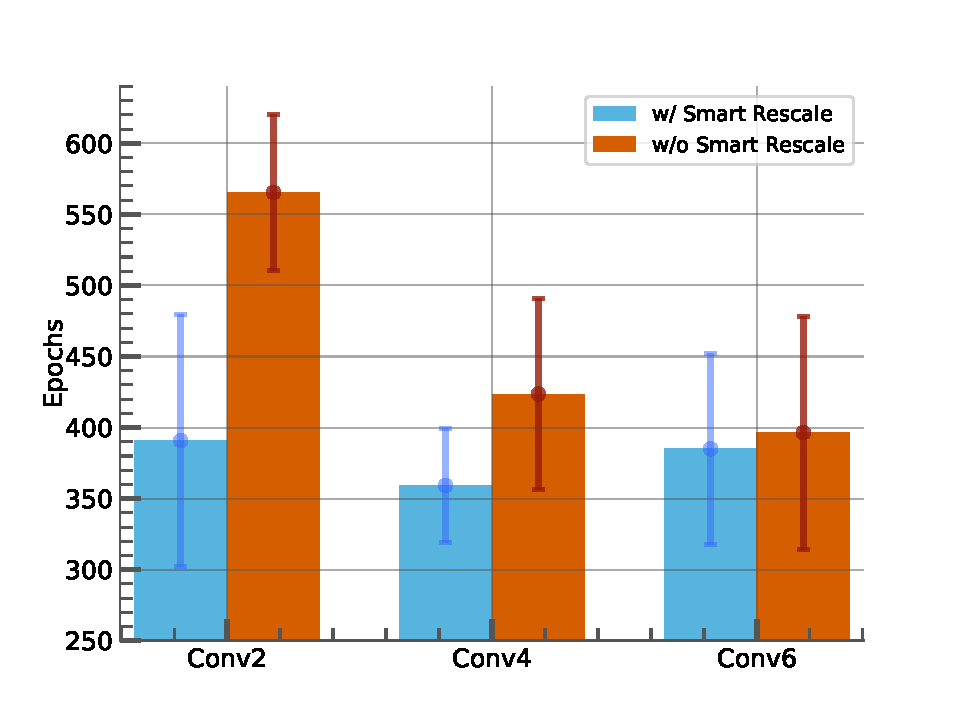
\includegraphics[width=0.49\textwidth]{chapter_2/assets/sr_impact_on_epochs_cifar10.pdf}}
\subfloat[CIFAR-100\label{fig:chap2:rescale_cifar100}]{
  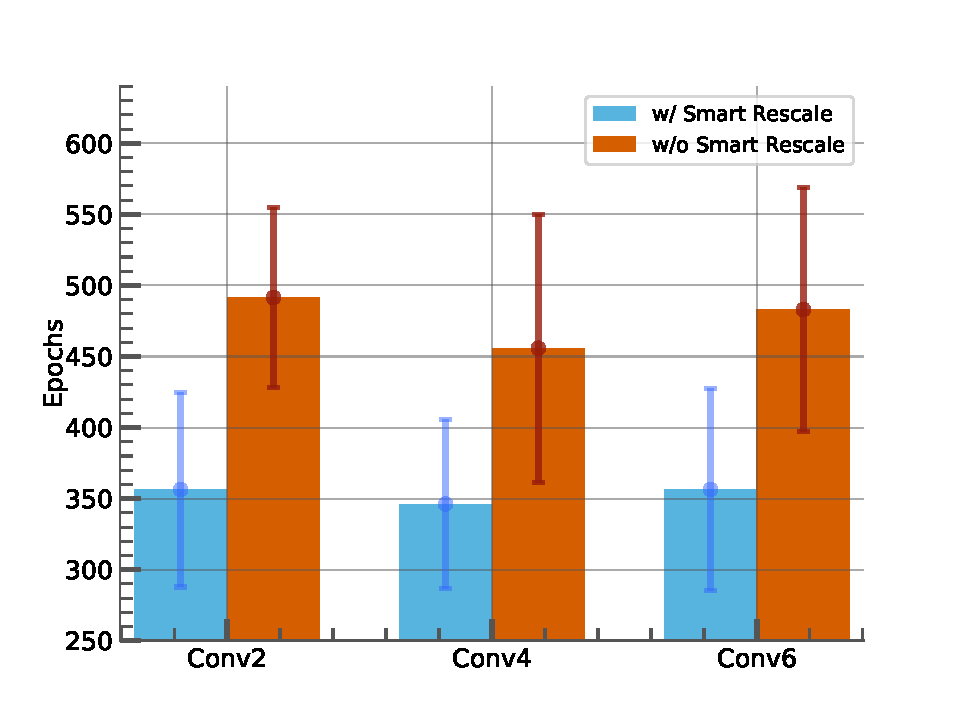
\includegraphics[width=0.49\textwidth]{chapter_2/assets/sr_impact_on_epochs_cifar100.pdf}}
\caption{Impact of \acf{SR} on the number of epochs required to reach
convergence for Conv\{2,3,4\} on CIFAR-10 and CIFAR-100.}
\label{fig:chap2:rescale_impact}  
\end{figure}


\subsection{Increasing sparsity a posteriori}
\label{sec:chap2:increasing_sparsity}

Unlike \cite{DBLP:conf/cvpr/RamanujanWKFR20}, the proposed \ac{ASLP} approach
does not enforce a predefined pruning rate during training. Instead, it allows
the network to determine its best pruning rate by updating weight probabilities
through backpropagation. The average pruning rate can be obtained by
thresholding the probabilities of selection, which is explained in
\cref{sec:chap2:performances}. The observed pruning rates are reported in
\cref{tab:chap2:observed_sparsity}, and they are typically around 50\%. However,
higher or lower pruning rates can be achieved by pruning weights based on their
associated selection probability (i.e., the associated mask $\bm{\hat{m}}$),
which enforces the pruning rate a posteriori and treats selection probabilities
as saliency scores during pruning. Notably, even with this a posteriori pruning
rate enforcement, Conv\{2,4,6\} networks trained with \ac{ASLP} achieve impressive
performances on CIFAR-10 and CIFAR-100 datasets for higher pruning rates than
their observed pruning rate, as shown in \cref{fig:chap2:sparsity_impact}. In
this figure, the solid line represents the average test accuracy of five
independent runs, and the shaded area represents plus or minus one standard
deviation.\\

Moreover, the results presented in \cref{fig:chap2:sparsity_impact} provide
further support for the \textit{thresholding} strategy. The pruning achieved by
the \textit{thresholding} strategy is comparable to the optimal pruning rate
found in this section through computationally expensive search methods (as done
in \cite{DBLP:conf/cvpr/RamanujanWKFR20}) across the tested architectures.

\begin{figure}[htbp]
\centering
\subfloat[cifar10\label{fig:chap2:sparsity_cifar10}]{
  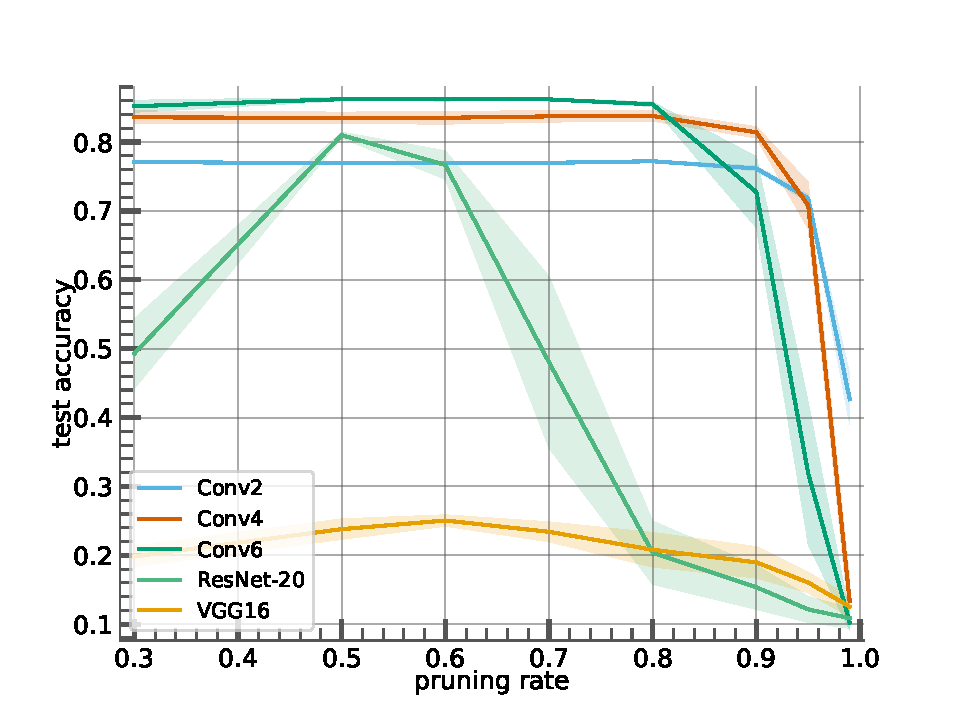
\includegraphics[width=0.49\textwidth]{chapter_2/assets/impact_of_pr_cifar10.pdf}}
  \subfloat[cifar100\label{fig:chap2:sparsity_cifar100}]{
  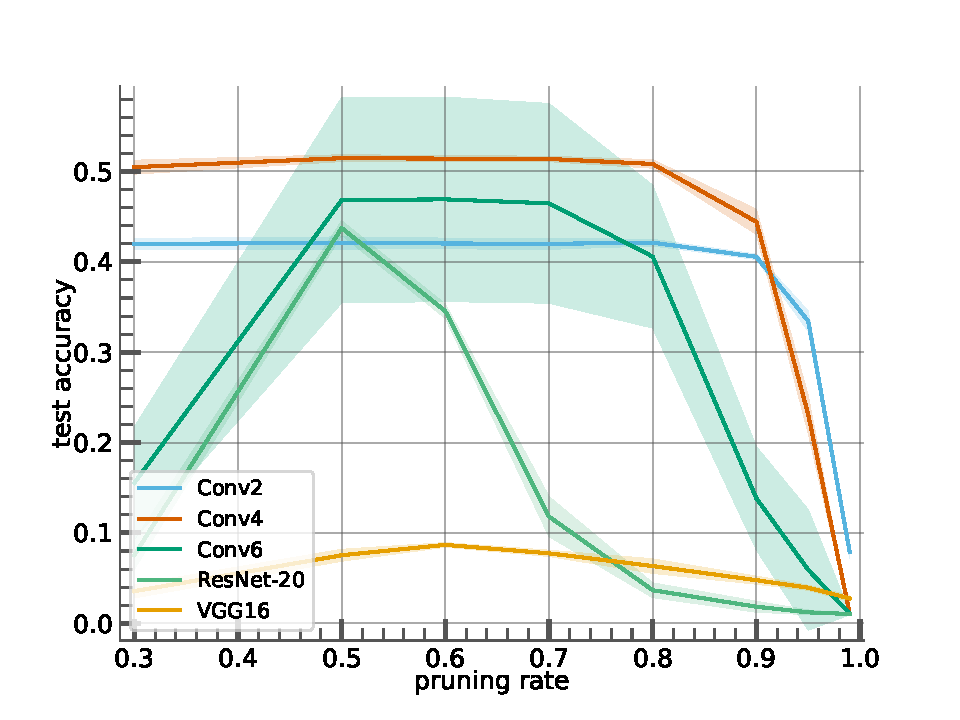
\includegraphics[width=0.49\textwidth]{chapter_2/assets/impact_of_pr_cifar100.pdf}}
  \caption{Comparative analysis of ASLP performance for CIFAR-10 and CIFAR-100
  datasets using various network architectures (Conv\{2,4,6\}, ResNet-20, and
  VGG16) at different pruning rates. ASLP performances are evaluated with
  \ac{WR}, \ac{SC} and data augmentation. Results demonstrate that Conv\{2,4,6\}
  networks maintain strong performance even at higher pruning rates and indicate
  that the pruning rate achieved by thresholding is optimal or near-optimal.}
\label{fig:chap2:sparsity_impact}
\end{figure}

\subsection{Optimal learning rate value}
\label{sec:chap2:impact_learning_rate}
The learning rate is an essential hyperparameter for training neural networks,
and a large learning rate typically results in divergence. However, in the case
of ASLP, increasing the learning rate as much as desired does not cause
divergence. It is worth noting that stability is not dependent on the learning
rate. A high learning rate converges more quickly, exhibiting better performance
initially, but is eventually outperformed if the training persists for an
extended period. Conversely, an excessively low learning rate may not reach
satisfactory performance levels in a reasonable amount of time, if at all. Our
experimental findings indicate that varying the learning rate does not affect
performance. In other words, opting for a high learning rate and subsequently
decreasing it yields worse results than maintaining a lower, constant learning
rate. We found that a learning rate of 50 strikes the optimal balance between
performance and training speed. Interestingly, this learning rate remains
consistent across all architectures and datasets.\\

\Cref{fig:chap2:lr_impact} shows the evolution of the test accuracy for Conv4,
VGG16 and ResNet-20 on CIFAR-10. The solid line represents the average of five
independent runs and the shaded area of the corresponding colour indicates the
range of $\pm$ one standard deviation. For ease of visualization, sequences have
been padded with their final values up to 1000 epochs. Networks have been
trained with data augmentation, \ac{WR} and \ac{SC}.\\

The robustness of ASLP to substantial learning rates can be attributed to the
fact that the trained masks, denoted by $\bm{\hat{m}}$, can be interpreted as
probabilities of selection by applying a sigmoid function (refer
\cref{sec:chap2:stochastic-sampling,prop:chap2:probability-interpretation}). The
sigmoid function is bounded between 0 and 1, ensuring that a large learning rate
does not cause the network output or \ac{SGD} gradients
to assume extremely large or even \ac{nan} values. Instead, it assigns very high or
very low values to $\bm{\hat{m}}$, resulting in probabilities of selection close
to 0 or 1. Due to the vanishingly small gradients as the masks move further away
from the origin, it is practically impossible to reactivate those weights, let
alone reactivate them with a smaller learning rate. This accounts for the
observation that reducing the learning rate after using a high learning rate
does not enhance performance.\\

\begin{figure}[htbp]
\centering
\subfloat[Conv4\label{fig:chap2:lr_conv4}]{
  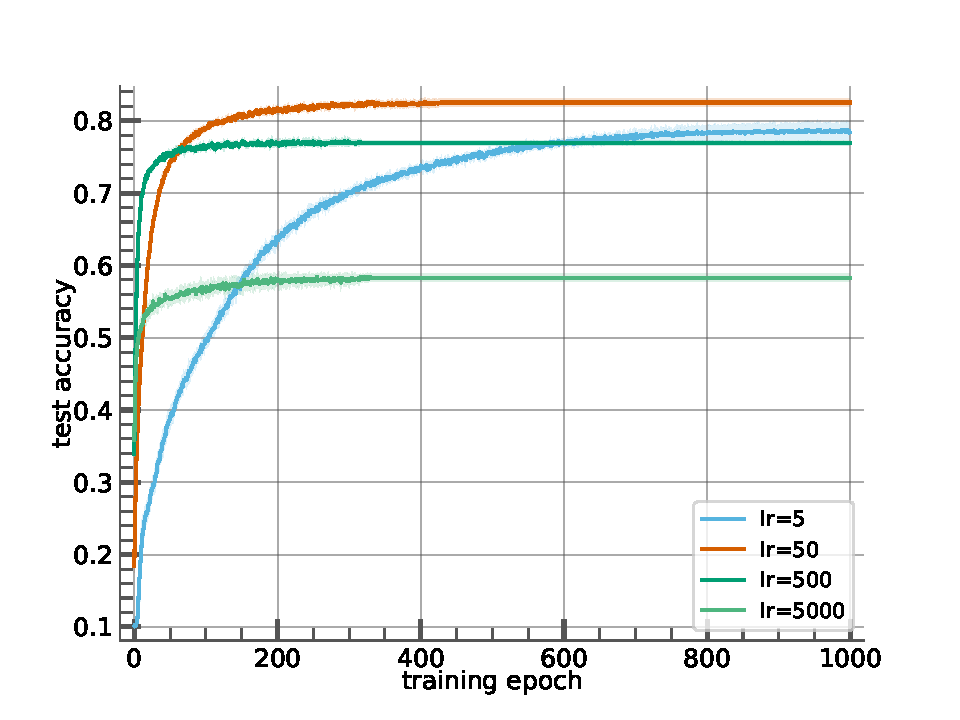
\includegraphics[width=0.33\linewidth]{chapter_2/assets/impact_of_lr_Conv4.pdf}}
  \subfloat[VGG16\label{fig:chap2:lr_vgg16}]{
  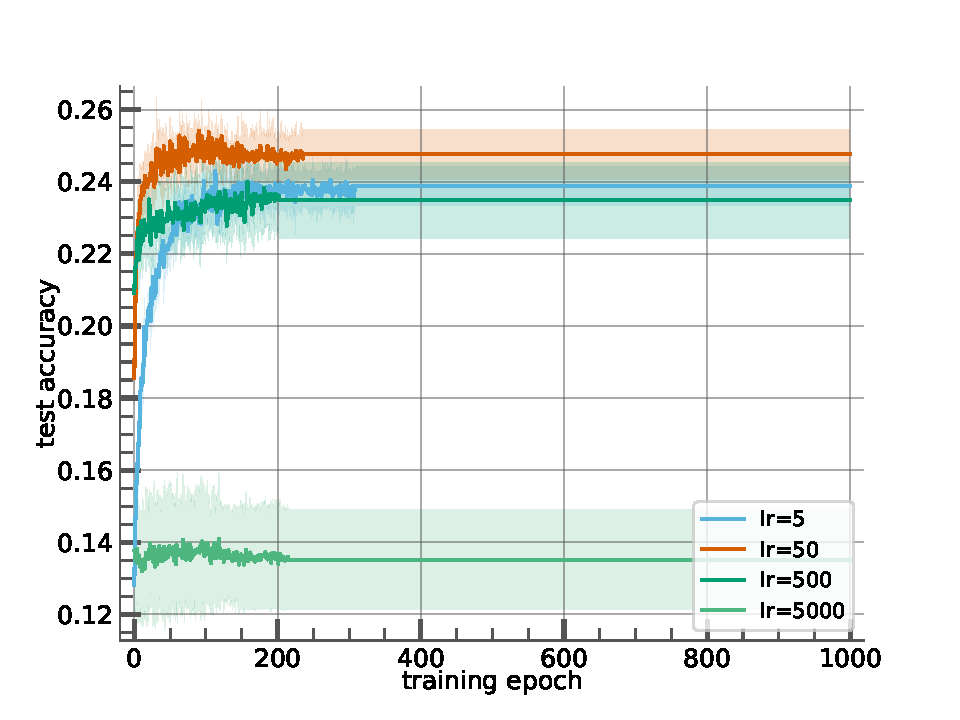
\includegraphics[width=0.33\linewidth]{chapter_2/assets/impact_of_lr_PrunableVGG16.pdf}}
  \subfloat[ResNet-20\label{fig:chap2:lr_resnet20}]{
  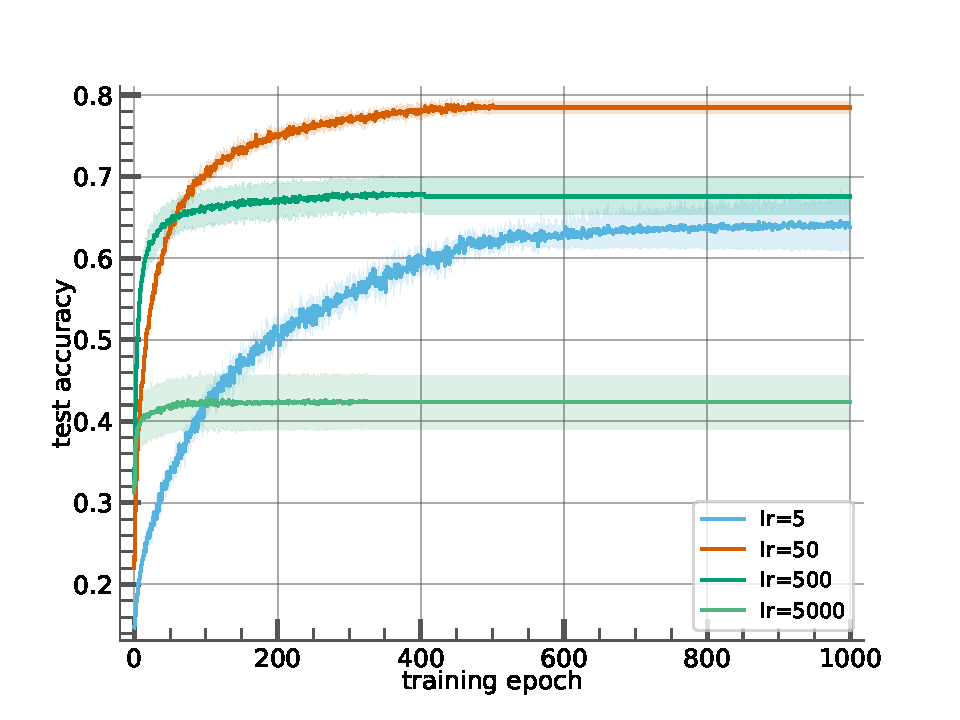
\includegraphics[width=0.33\linewidth]{chapter_2/assets/impact_of_lr_PrunableResNet20.pdf}}
  \caption{Evolution of the test accuracy for Conv4, VGG16 and ResNet-20 trained
  with ASLP (with data augmentation, \ac{WR} and \ac{SC}) on CIFAR-10 for various learning
  rates. A learning rate of 50 yields the optimal balance between performance
  and training speed.}
\label{fig:chap2:lr_impact}
\end{figure}

% endregion: experiments

\section{Conclusion}
% region : Conclusion

In this chapter, we introduced the \acl{ASLP} method, which focuses on selecting
efficient subnetworks from large, untrained neural networks through stochastic
pruning, without training the weights. \acl{ASLP} is a stochastic subnetwork selection
method that uses \acl{GS} sampling and a new mask parametrisation to
optimize the subnetwork topology while mitigating numerical instabilities.
Additionally, we presented the \acl{SR} technique to accelerate training and
improve the accuracy of the resulting subnetworks. Our experimental results show
that ASLP outperforms state-of-the-art methods, such as Edge-popup
\cite{DBLP:conf/cvpr/RamanujanWKFR20} and Supermask
\cite{DBLP:conf/nips/ZhouLLY19}, on the CIFAR-10 and CIFAR-100 datasets across
various network architectures. The proposed \textit{thresholding} pruning
strategy consistently yields better performance than Supermask's
\textit{averaging} approach. Furthermore, our \acl{SR} method leads to faster
convergence and improved accuracy compared to other weight-rescaling techniques,
such as \acl{DWR}. \acl{ASLP} also exhibits robustness to substantial learning
rates, ensuring stable performance across different network architectures and
datasets.\\

All in all, the \acl{ASLP} method provides a promising solution for selecting
efficient subnetworks from large untrained neural networks through stochastic
pruning, offering improved performance and faster convergence. 

% TODO: ajouter la partie qui lie le prochain chapitre.

\textit{Ajouter la partie qui lie le prochain chapitre.}

%endregion : conclusion
